\documentclass[conference]{IEEEtran}
\usepackage{cite}
\usepackage{balance}
\usepackage{graphicx}

\usepackage{xspace}
\newcommand{\ie}{{\emph{i.e.}},\xspace}
\newcommand{\viz}{{\emph{viz.}},\xspace}
\newcommand{\eg}{{\emph{e.g.}},\xspace}
\newcommand{\etc}{etc.}
\newcommand{\etal}{{\emph{et al.}}}

\usepackage{amssymb}
\newcommand{\nnbb}[2]{
    \fbox{\bfseries\sffamily\scriptsize#1}
    {\sf\small$\blacktriangleright$\textit{#2}$\blacktriangleleft$}
   }

\newcommand{\as}[1]{\nnbb{Alexander}{#1}}
\newcommand{\bv}[1]{\nnbb{Bogdan}{#1}}
\newcommand{\vf}[1]{\nnbb{Vladimir}{#1}}
\newcommand{\yz}[1]{\nnbb{Yangyang}{#1}}

\begin{document}

\title{Census of Software Engineering Practices
Following Adoption of Continuous Integration}

\author
{\IEEEauthorblockN{}
\IEEEauthorblockA{}
}
\maketitle
\begin{abstract}
Continuous Integration (CI) has become a key part of the devops ideology of mashing development and operations together to shorten the cycles of delivering a product to users. CI has become a disruptive innovation in software development: with proper implementation, e.g. Travis CI or Jenkins CI, and adoption, positive effects have been demonstrated on pull request throughput and scaling up of project sizes. As any other innovation, adopting it implies adapting existing practices in order to take full advantage of its potential. Here we study the adaptation and evolution of code writing, review practices and unit testing practices as Travis CI is adopted by XX established projects on GitHub. By employing a mix of quantitative studies and case studies we triangulate the general evolution trajectories, and provide reasoning for the differences encountered among the projects.
\end{abstract}

\section{Introduction}
Devops, or bringing development and build/release activities in the same framework can bring changes in the product to the user-plane more quickly. For it to be effective, the technology that implements these ideas has to allow for a seamless back and forth between development, integration, code testing review, and release. 

Continuous Integration is the part of devops that seamlessly builds, tests, and integrates developer changes, and performs any pre-specified testing. CI (\eg Travis CI, Jenkins CI, Hudson CI), if implemented properly, can benefit the distributed software development process, in particular code change throughput~\cite{Stolberg} and some aspects of code quality~\cite{VasilescuYWDF15}. It is a disruptive technology, in that it can scale up distributed development without noticeable diminishment in quality.

Proper implementation is key here, otherwise the benefits may not be felt, and the technology may become a drag on resources, since it subsumes continuous builds and testing. 
This is particularly true in team environments, where it falls to each individual developer to keep up with project specific implementation policies.
For that reason, Martin Fowler wrote an article on CI best practices~\cite{}, which has been very influential and in many projects there are expectations that those practices define CI and that they will be followed.~\cite{}
In particular, those practices are: Maintain a Single Source Repository,  Automate the Build, Make Your Build Self-Testing, Everyone Commits To the Mainline Every Day, Every Commit Should Build the Mainline on an Integration Machine, Fix Broken Builds Immediately, Keep the Build Fast, Test in a Clone of the Production Environment, Make it Easy for Anyone to Get the Latest Executable, Everyone can see what's happening, and Automate Deployment.
But to what extent are they followed in practice?

In this paper we sought to examine the extent to which best practices of CI are actually transitioned to and followed, after CI adoption in online software development projects.  We focus on three major aspects of modern development: practices related to code changes, code testing, and code reviews, and operationalize them into measures for them which we observe from data of GitHub repositories.
We introduce regression discontinuity desing analyses in order to evaluate the effect of an intervention, in our case CI adoption, on the transition toward expected behaviors in the above three practices.
Applying those methods to hundreds of projects, appropriately selected, we find that:

\begin{itemize}

\item There is a significant and persistent downward trend in commit churn after CI is adopted, over all projects, but also for a large fraction of individual projects. This trend is non-existent before the adoption.

\item Consistent with the above, we also find that the number of commits and PRs increases after CI adoption, and is random before it.

\item There is a rapidly increasing trend in the number of automatic test per PR after CI adoption.

\item There are significantly more issues submitted after CI adopted than before.

\item There are no significant changes in the frequency of commits after CI adoption.
\end{itemize}


In what follows, we tell this paper's story in a carefully crafted, yet mostly standard multisectioned format, beginning with the inimitable background and theory section, followed by an examplary part on methodology, culminating in our tight results and logical discussion, with our long reaching conclusions, and the unavoidable threats to validity section bringin up the rear.


\section{Background and Theory}

For a developer not proficient with the operations side of the process, transitioning to an integrated CI platform, like Travis CI, involves adaptation of their established processes to the new environment. During this transition, some developers will experience a more streamlined process evolution trajectory than others. Studying those trajectories can provide lessons learned.


We expect the following to potentially change in the transition <need to write theory behind each>:

On the developer side:
Change in code writing/committing: we expect smaller change sets over time
We expect More unit testing over time
Operations side:
More discussions in code review over time
Different categories of initial faults

Continuous integration encourages developers to ``break down their work into small chunks of a few hours each'', as smaller and more frequent commits keep them to keep track of their progress and reduces the debug effort~\cite{Fowler,Duvall}. %Duvall [p. 31,38,40]
Therefore, in \textbf{RQ1} we investigate whether introduction of the continuous integration has indeed led to smaller commits.
\as{Why do not we look at their frequency? In an early study Miller has observed that on average Microsoft developers committed once a day, while off-shore developers committed less frequently due to network latencies~\cite{Miller}; Y\"{u}ksel reports 33 commits per day~\cite{Yuksel}.}

RQ1: Are developers reducing the size of code changes in each commit post CI adoption? Do they continue to do so over time?

Moreover, continuous integration is closely related to presence of automated tests~\cite{Fowler}. Duvall even claims that continuous integration without such tests should not be considered continuous integration at all~\cite{Duvall}, while Cannizzo, Clutton and Ramesh deem an extensive suite of unit and acceptance tests to be an essential first step~\cite{CannizzoCluttonRamesh}. \as{Y\"{u}ksel reports increase of the number of automated tests but they have combined introduction of CI with automated testing~\cite{Yuksel}. }

RQ2: How are developers transitioning to automated testing over time?

For continuos integration to have the stated benefits, code review should play a prominent role. In a pull-request model of development, code review is done through comments in open issues.

RQ3: Are developers transitioning to using more issues after the adoption of CI?


%\subsection{RQs}

\section{Methods}

a) data gathering

b) data description

c) analysis methods

- Regression discontinuity design




- Statistical models

- boxplots

- case studies



\section{Results and Discussion}

\subsection{RQ1: Changes in Code Churn Practices}

Data: 567 projects with 500+ nonmerge commits

Fig 1: Box plots of code churn per unit time period, one for each time point, each point an aggregate of all projects



\begin{figure}[!t]
\centering
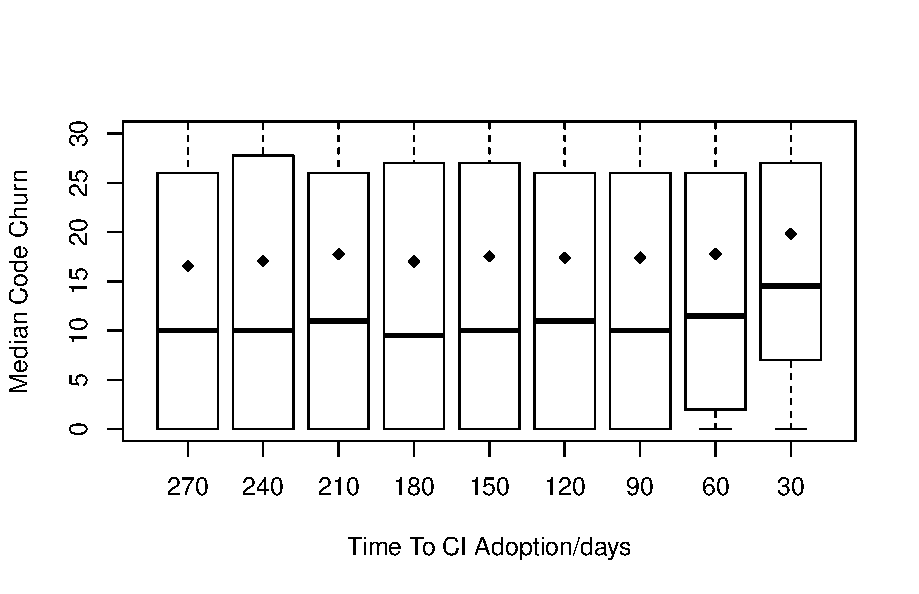
\includegraphics[width=0.5\textwidth]{churn_before.pdf}
\caption{The Code churn before CI adoption}
\label{Fig:CodeChurnBefore}
\end{figure}



\begin{figure}[!t]
\centering
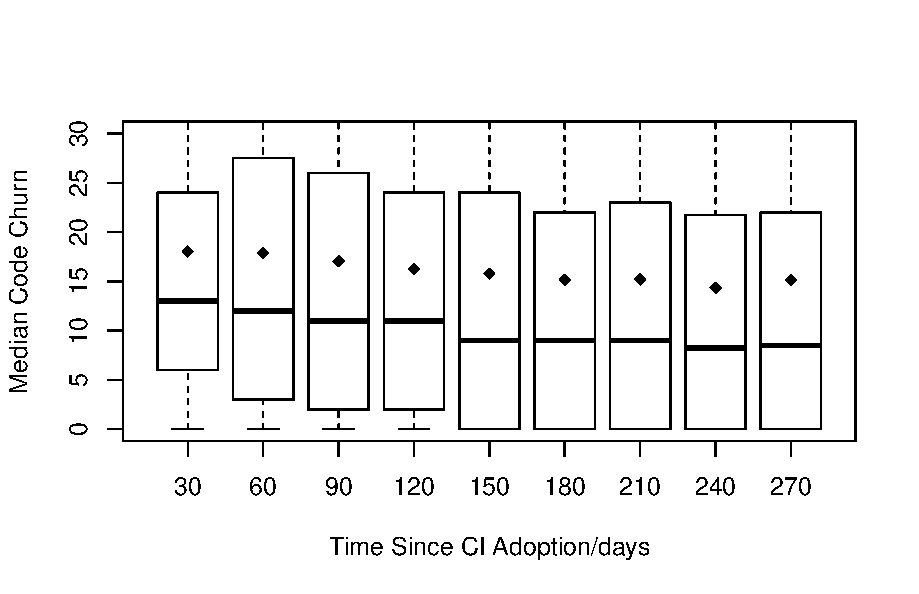
\includegraphics[width=0.5\textwidth]{churn_after.pdf}
\caption{The Code churn after CI adoption}
\label{Fig:CodeChurnAfter}
\end{figure}

Table 1: Summary of all models

Table 2: Projects with negative trends after CI

\subsection{RQ2: Changes in Issues}

Fig 2: Box plots of \# issues per unit time period, one for each time point, each point an aggregate of all projects





\subsection{RQ3: Trends in Unit Testing Per Pull Request}




Fig 3: Box plots of fraction of builds with tests or unit tests per pull request, per unit time period, one for each time point, each point an aggregate of all projects

% !TEX root = CI_Adoption.tex
\section{Related Work}
\label{sec:rw}
Adoption and impact of continuous integration have attracted \as{limited/extensive} attention from the research community. Already in 2003 based on the studies of FreeBSD and Mozilla Holck and J{\o}rgensen have observed that continuous integration, interpreted as distributed development and obligation to integrate one's own contributions, is capable of replacing traditional software engineering coordination mechanisms~\cite{HolckJ03}.  
Deshpande and Riehle have studied adoption of continuous integration based on Ohloh.net data~\cite{Deshpande2008}. Assuming that the use of continuous integration reduces the size of commits, they have studied the size of commits in 5122 projects and, since no commit size reduction has been observed, they have concluded that continuous integration has not been used. Their observations might have been affected by lack of actual relation between presence of continuous integration and commit size, aggregation effect of considering the average commit size over different projects as well as the period studied (January 1990--December 2006). 

Ease of use of the Travis-CI~\cite{TravisCI} continuous integration system led to its popularity on GitHub and triggered a series of research studies~\cite{era14,VasilescuYWDF15,yue2015wait,BellerGZ16,Hilton2016,Yu2016}.\as{To be continued. Maybe Bogdan can write about his own work.}

Industrial adoption of continuous integration systems has been recently studied in several papers~\cite{Leppanen2015,Laukkanen2015Agile,Debbiche2014,Stahl2014ICSEComp,Stahl2014JSS} and is a subject of the recent survey by Eck, Uebernickel and Brenner~\cite{EckUB14}. However, this line of work is based on interviews rather than on analysis of the development data.

\as{Miller~\cite{Miller} discusses build breaks, is this relevant?}
\as{Van der Storm discusses backtracking as a way of addressing build failures~\cite{Storm2008}.}
\as{Laukannen and M\"{a}ntyl\"{a} have surveyed three papers discussing the impact of the build waiting times. Some of the consequences of the long/short build waiting times are related to CI~\cite{Laukkanen2015RCSE}.}


\section{Conclusion}

\begin{figure}[!t]
\centering
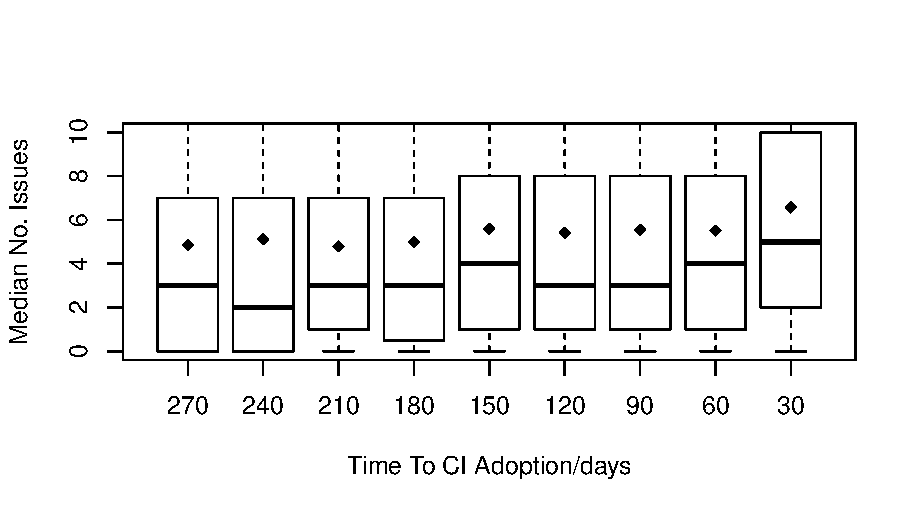
\includegraphics[width=0.5\textwidth]{issues_before.pdf}
\caption{Median number of issues before CI adoption}
\label{Fig:IssuesBefore}
\end{figure}


\begin{figure}[!t]
\centering
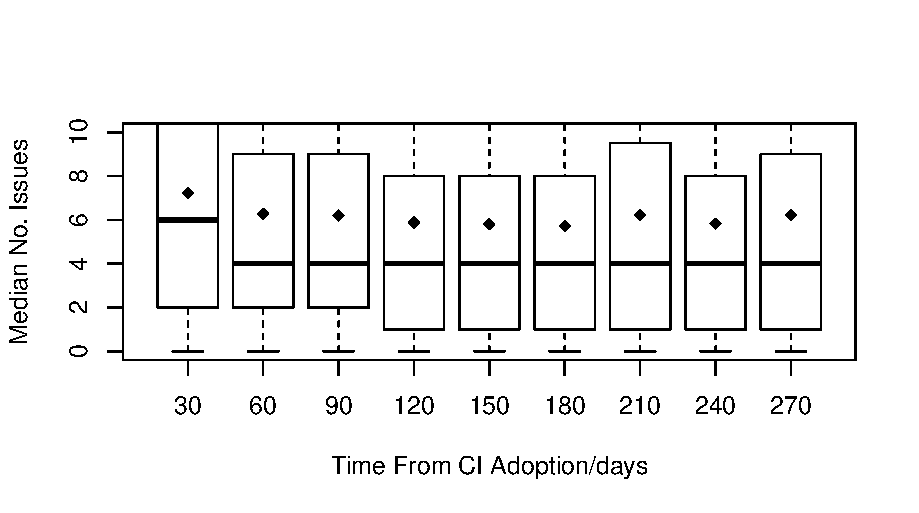
\includegraphics[width=0.5\textwidth]{issues_after.pdf}
\caption{Median number of issues after CI adoption}
\label{Fig:IssuesAfter}
\end{figure}


\begin{figure}[!t]
\centering
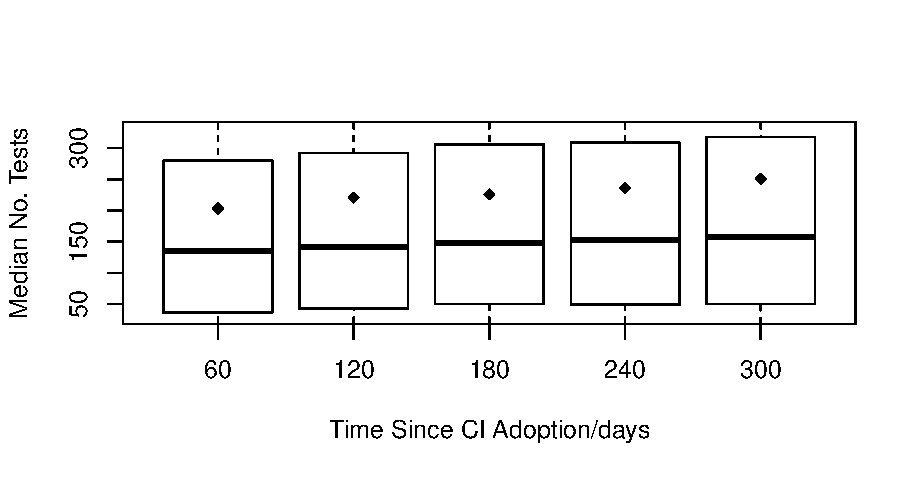
\includegraphics[width=0.5\textwidth]{tests.pdf}
\caption{Unit tests per build following CI adoption}
\label{Fig:Tests}
\end{figure}

\section{Threats to Validity}

\bibliographystyle{IEEEtran}
\bibliography{references}

\end{document}